\begin{proof}
  By applying the chain rule to $e^{\log z} = z$, we find that $\frac{d}{dz}\log z = \frac{1}{z}$.

  We can check hat the given power series has radius of convergence $1$. We have that:
\[
\frac{d}{dz} \log (1+z) = \frac{1}{1+z}\mpunct{,}
\]
but we also have that:
\[
\frac{d}{dz}\left(\sum_{n\geq 1} (-1)^{n-1}\frac{z^n}{n}\right) = \frac{1}{1+z} \mpunct{.}
\]
Now evaluate at $0$ to check the expressions agree.
\end{proof}

\paragraph{Heuristic remark}

Instead of slitting the plane, one could view $\log$ as a multi-valued function $z \mapsto \{ \ln \abs{z} + i\theta \mid \theta \text{ is any value of } \arg z\}$. 
A point $p \in \CC$ such that the multi-valued function $f$ has no continuous single-value branch in any neighbourhood $B_\epsilon(p) \setminus \{p\}$ is called a branch point\index{branch point} of $f$.
For example, $0$ is a branch point of $\log$. We can set $z^\alpha = e^{\alpha\log z}$ and hence define for example $\sqrt{z}$ either as a function on a slit plane, or as a multi-valued function with branch point at $0$.
To resolve the problem of branch points, it is possible to say that $\log$, $z^{1/2}$ are well-defined on certain Riemann surfaces (spaces mapping to $\CC^*$).

\section{Contour integrals}
Let $f : [a, b] \rightarrow \CC$. We say $f$ is (Riemann) integrable\index{integrable} if $\Re f$ and $\Im f$ are integrable. We define
\[
\int_a^b f(t)dt = \int_a^b\Re f (t) dt + i\int_a^b \Im f(t) dt \mpunct{.}
\]

\begin{proposition}
\[
\abs*{\int_a^b f(t) dt} \leq (b-a)\sup_t\abs*{f(t)} \mpunct{,}
\]
with equality if and only if $f$ is constant.
\end{proposition}

\begin{proof}
  let $\theta = \arg \int_a^b f(t) dt$, and let $M = \sup\abs{f(t)}$. We have that:
\begin{IEEEeqnarray*}{rCl}
\abs*{\int_a^b f(t)} &=& \int_a^b e^{-i\theta}f(t) dt \\
&=& \int_a^b \Re (e^{-i\theta} f(t)) dt \quad \text{ as we know that the previous line is real} \\
&\leq& \int_a^b \abs{f(t)} dt \\
&\leq& (b-a)M \mpunct{.} 
\end{IEEEeqnarray*}
We have equality if and only if $\abs{f(t)} = M$ and $\arg f(t) = \theta$, i.e. $f$ is constant.
\end{proof}

\begin{definition}
  A path\index{path} is a $C^1$-smooth (or just smooth) map $\phi : [a, b] \rightarrow \CC$. A path is said to be simple\index{simple (path)} if there are no self-intersections except (possibly) at the end points, i.e.
\[
\phi(t_1) = \phi(t_2) \Rightarrow \{t_1, t_2\} = \{a, b\} \text{ or } t_1 = t_2 \mpunct{.}
\]
A simple closed path is called a contour\index{contour}.
\end{definition}

If $\gamma : [a, b] \rightarrow \CC$ is $C^1$-smooth, we let:
\[
\text{length}(\gamma) = \int_a^b \abs*{\gamma'(t)} dt\mpunct{.}
\]

\begin{definition}
  Given $\gamma : [a, b] \rightarrow U \subseteq \CC$  path, and $f : U \rightarrow \CC$ continuous, we define:
\[
\int_\gamma f(z) dz = \int_a^b f\left(\gamma(t)\right)\gamma'(t) dt
\]
\end{definition}

\paragraph{Easy properties}

\begin{enumerate}
\item Integrating along some fixed path $\gamma$ is linear in the function $f$.
\item If $-\gamma$ denotes the path $\gamma$ traversed in the opposite direction, then:
\[
\int_{-\gamma} f(z)dz = -\int_\gamma f(z) dz \mpunct{.}
\]

\item The integral along $\gamma$ is independent of the parametrisation of the path. 
Indeed, let $\phi : [a', b'] \rightarrow [a, b]$ be $C^1$ with $\phi(a') = a$ and $\phi(b') = b$. 
Then if $\delta = \gamma \circ \phi$, we claim:
\[
\int_\delta f(z) dz = \int_\gamma f(z) dz \mpunct{.}
\]
We have the following:
\[
  \int_{a'}^{b'} f(\gamma(\phi(t)))\gamma'(\phi(t))\phi'(t) dt = \int_a^b f(\gamma(u))\gamma'(u) du
\]
where we have set $u = \phi(t)$.
\end{enumerate}

\paragraph{Remark}

If $\gamma$ is only piecewise $C^1$ smooth, we define:
\[
\int_\gamma f(z)dz = \sum_i \int_{\gamma_i} f(z)dz 
\]
where $\gamma = \gamma_1 * \gamma_2 * \dotsb * \gamma_r$ is a concatenation of smooth $\gamma_i$. 
Integration is additive in the sense that, if $a < \tilde{a} < b$, then we have:
\[
\int_\gamma f(z)dz = \int_{\gamma\rvert_{[a, \tilde{a}]}} f(z)dz + \int_{\gamma\rvert_{[\tilde{a}, b]}} f(z) dz \mpunct{.}
\]

\paragraph{Example}

Let $f(z) = z^n$ defined on $U = \CC^*$, and let $\gamma : [0, 2\pi] \rightarrow U$ such that $\gamma(\theta) = e^{i\theta}$. Then, we have that:
\[
\int_\gamma f(z) dz = \begin{cases}2\pi{}i & \text{if } n = -1 \mpunct{,} \\0 & \text{otherwise.}\end{cases}
\]

\begin{proof}
  We have the following:
\[
\int_\gamma f(z)dz = \int_0^{2\pi}e^{in\theta}ie^{in\theta}d\theta = i\int_0^{2\pi} e^{i(n+1)\theta}d\theta \mpunct{.}
\]
Hence, if $n = -1$, we get $2\pi{}i$. If $n \neq -1$, we have that $\left[\frac{e^{i(n+1)\theta}}{n+1}\right]_0^{2\pi} = 0$.
\end{proof}

\paragraph{Example}
\begin{figure}
  \centering
   \begin{tikzpicture}[scale=0.75]
    \tkzInit[xmin=-5,xmax=5,ymin=-1,ymax=5]

    \tkzDefPoint(0,0){O}
    \tkzDefPoint(-4,0){A}
    \tkzDefPoint(4,0){B}

    \tkzDefPoint(-5,0){xmin}
    \tkzDefPoint(5,0){xmax}

    \tkzDefPoint(0,5){ymax}
    \tkzDefPoint(0,-1){ymin}

    \tkzDrawSegment(xmin,xmax)
    \tkzDrawSegment(ymin,ymax)

    \tkzDrawArc[color=blue](O,B)(A)
    \tkzDrawSegment[color=blue](B,A)

    \tkzLabelPoint[below](A){$-R$}
    \tkzLabelPoint[below](B){$R$}

  \end{tikzpicture}

  \caption{half-circle of radius $R$}
  \label{fig:4.1}
\end{figure}

Let $\gamma$ be as in the figure\ref{fig:4.1}, and $f(z) = z^2$. We write $\gamma = \gamma_1 * \gamma_2$, with $\gamma_1 : [-R, R] \rightarrow \CC$ such that $\gamma_1(t) = t$ and with $\gamma_2 : [0, 1] \rightarrow \CC$ such that $\gamma_2(t) = Re^{i\pi{}t}$.
Then we have the following:
\begin{IEEEeqnarray*}{rCl}
\int_\gamma f(z) dz &=& \int_{-R}^R t^2dt + \int_0^1 R^2e^{2\pi i t} i \pi R e^{i \pi t} dt \\
&=& \frac{2R^3}{3} + R^3 i \pi \int_0^1 e^{3\pi i t} dt \\
&=& \frac{2R^3}{3} - \frac{2R^3}{3} \\
&=& 0 \mpunct{.}
\end{IEEEeqnarray*}

\begin{proposition}
  For a path $\gamma : [a, b] \rightarrow U$ and $f : U \rightarrow \CC$ continuous, we have that:
\[
\abs*{\int_\gamma f(z) dz} \leq \text{length}(\gamma) \sup_\gamma \abs*{f(z)} \mpunct{.}
\]
\end{proposition}

\begin{proposition}
  Let $f : U \rightarrow \CC$ be continuous, and suppose that there exists $F : U \rightarrow \CC$ such that $F'(z) = f(z)$ for all $z \in U$. Then if $\gamma : [a, b] \rightarrow U$, we have that:
\[
\int_\gamma f(z) dz = F(\gamma(b)) - F(\gamma(a)) \mpunct{.}
\]
\end{proposition}

\begin{proof}
  We have that:
\[
\int_\gamma f(z) dz = \int_a^b f(\gamma(t))\gamma'(t) dt = \int_a^b(F \circ \gamma)'(t) dt \mpunct{.}
\]
\end{proof}

$F$ is called an antiderivative\index{antiderivative} of $f$ on $U$.

%%% Local Variables: 
%%% mode: latex
%%% TeX-master: "complex_analysis"
%%% End: 
